\documentclass{article}


\usepackage[english]{babel}
\usepackage{listings}

\usepackage[letterpaper,top=2cm,bottom=2cm,left=3cm,right=3cm,marginparwidth=1.75cm]{geometry}

% Useful packages
\usepackage{amsmath}
\usepackage{graphicx}
\usepackage[colorlinks=true, allcolors=blue]{hyperref}
\usepackage{listings}
\lstset{language=Python}

\title{COSC 343: homework 3}
\author{Micah Sherry}

\begin{document}
\maketitle
\section{four point Gaussian quadrature rule on [-1, 1]}
\subsection{defining four point Gaussian quadrature}
	Define a four point Gaussian Quadrature rule on the interval [-1,1].
	\\To define the four point Gaussian quadrature rule I solved (using sage) the system:
	$$ w_1 + w_2 + w_3 + w_4 = 2 $$
	$$ w_1x_1 + w_2x_2 + w_3x_3 + w_4x_4 = 0 $$
	$$ w_1x_1^2 + w_2x_2^2 + w_3x_3^2 + w_4x_4^2 = \frac{2}{3} $$
	$$ w_1x_1^3 + w_2x_2^3 + w_3x_3^3 + w_4x_4^3 = 0 $$
	$$ w_1x_1^4 + w_2x_2^4 + w_3x_3^4 + w_4x_4^4 = \frac{2}{5} $$
	$$ w_1x_1^5 + w_2x_2^5 + w_3x_3^5 + w_4x_4^5 = 0 $$
	$$ w_1x_1^6 + w_2x_2^6 + w_3x_3^6 + w_4x_4^6 = \frac{2}{7} $$
	$$ w_1x_1^7 + w_2x_2^7 + w_3x_3^7 + w_4x_4^7 = 0 $$
	I got the solution (rounded to 4 decimal places for readability):
	$$\begin{pmatrix}
		w_1 \\	w_2 \\	w_3 \\	w_4 \\	x_1 \\	x_2 \\	x_3 \\	x_4 \\
	\end{pmatrix}
	\quad \approx \quad
	\begin{pmatrix}
		0.3479 \\0.6521 \\0.6521 \\0.3479 \\-0.8611 \\-0.34\\0.34 \\0.8611 \\
	\end{pmatrix}$$
	To use these points and weights to integrate numerically use the formula:
	$$\int_{-1}^{1}f(x)dx \approx \sum_{i=1}^{4}w_i\times f(x_i)$$
	\subsubsection*{Code:}
		\lstinputlisting[firstline=3,lastline=25]{../GaussianQuadrature.py}
\subsection{highest exactly integrable degree polynomial}
	What is the highest degree polynomial function that your rule can integrate exactly?
	\\Gaussian quadrature with n points should be able to integrate all polynomials of degree $2n-1$ exactly. This comes from the fact that Gaussian quadrature with n point has $2n$ unknown variables and needs $2n$ equations to solve and the last equation in the system  $$ w_1x_1^{2n-1} + ... +w_nx_n^{2n-1} = \int_{-1}^{1}x^{2n-1}dx$$ So a four point Gaussian quadrature routine should be able to integrate all polynomials of degree 7 or less.  
\subsection{test of four point Gaussian quadrature on [-1,1]}
	Write code that shows your four point Gaussian Quadrature rule on [-1,1] quadrature rule will in fact integrate polynomial of this degree exactly.
	\\To verify my code works i will be using the polynomial $$f_1(x)=2x^7 - 3x^6 + 5x^5 - 4x^4 + x^3 - 2x^2 + 3x - 1$$ and will be using the polynomial $$f_2(x)= x^6 $$
	\subsubsection*{Code:}
		\lstinputlisting{../test1.py}
	\subsubsection*{output:}
		For the first polynomial's true value I got:$$\int_{-1}^{1}f_1(x)dx= F_1(1)-F_1(-1)=-5.7904761904761894$$ 
		and using Gaussian quadrature I got a value of $-5.790476190476198$ \\\\
		For the second polynomial's true value I got:$$\int_{-1}^{1}f_2(x)dx= F_2(1)-F_2(-1)=0.2857142857142857$$ 
		and using Gaussian quadrature I got a value of $0.2857142857142867$ \\
\section{four point Gaussian quadrature on [a,b]}
	\subsection{defining four point Gaussian quadrature on [a,b]}
		Define a four point Gaussian Quadrature rule that can be used on the interval [a, b].\\\\
		to define the four point quadrature on the interval [a,b] I took the code from the quadrature routine on [-1,1] and created a function that linearly maps points on [a,b] to a point on [-1,1] and multiplies the weights by $\frac{b-a}{2}$ which is the slope of the line used to derive the the mapping function
	\subsubsection*{Code:}
		\lstinputlisting[firstline=25,lastline=41]{../GaussianQuadrature.py}
	\subsection{Testing}
		Show that your four point quadrature rule on [a,b] integrates the same degree polynomial as the one you had defined on [-1,1].\\\\
		\lstinputlisting{../test2.py}
		to see that given the same polynomial it will produce the same results i tested it on $\int_{-1}^1f_1(x)dx$ for that I got answer of $-5.790476190476198$ which is the same as my approximation above.\\
		then I tested it on a different integral (on a different interval) 
		$$\int_{-2}^{3} 12x^7 + x^4 - 10x^2+ 42x dx = 9500.833333333334$$
		 and the approximation I got was $9500.833333333345$.
		 


\section{Composite quadrature}
	Define a four point Gaussian composite quadrature rule. Use a non-polynomial test
	function and find the order of convergence of this four point Gaussian composite
	quadrature rule. \\\\
	I based my composite quadrature routine based on the formula: $$\sum_{i=0}^{n-1}Gauss(f,a_{i}, a_{i+1})$$. Where n is the number of intervals and the interval [A,B] is divided into the sub-intervals $[a_{i},a_{i+1}]$
	
	\subsubsection*{quadrature routines:}
		\lstinputlisting[firstline=25,lastline=54]{../GaussianQuadrature.py}
	\subsubsection*{rate of convergence and test function:}
		To find the formula for the rate of convergence we need  error terms.  the error terms are $O(h^{\alpha})$ which means:
		$$\epsilon_h = ch^{\alpha} \text{ and } \epsilon_{\frac{h}{2}} = c\left(\frac{h}{2}\right)^{\alpha}$$
		using those two equations we can find that 
		$$\alpha = \frac{ln\left(\frac{\epsilon_h}{\epsilon_{\frac{h}{2}}}\right)}{ln(2)}$$
		
		\lstinputlisting[firstline=54,lastline=62]{../GaussianQuadrature.py}
		To test the composite I approximated $$\int_{-10}^{2}x^2e^xdx$$ The exact value is $14.772573406430277$ and with my composite quadrature rule I got $14.77257340643028$ and using the find alpha method i found alpha to be 8
		\lstinputlisting{../test3.py}
		
		\begin{figure}[hbt!]
			\centering
			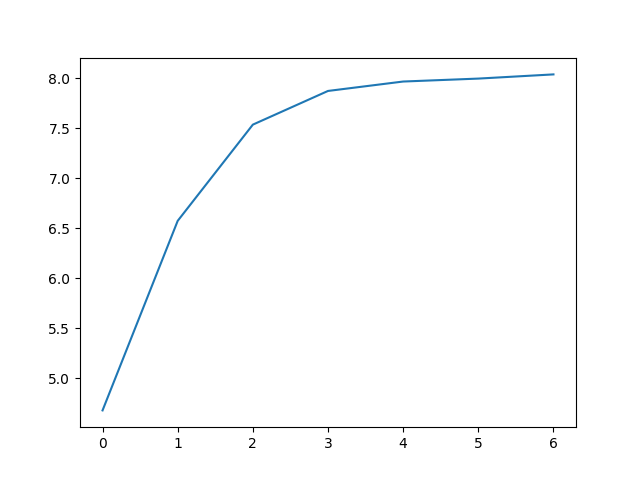
\includegraphics[width=.75\linewidth]{alpha_plot.png}
			\caption{convergence rate for composite quadrature}
			\label{fig:convergence rate for composite quadrature}
		\end{figure}
		

\end{document}